\documentclass[runningheads]{llncs}
\usepackage[T1]{fontenc}
\usepackage{amsmath,amssymb}
\usepackage{graphicx,booktabs,multirow,microtype,xcolor,array}
\usepackage{tikz,fontawesome5}
\usetikzlibrary{arrows.meta,positioning,calc,fit,backgrounds}
\usepackage{placeins}
\usepackage{algorithm}
\usepackage[noend]{algpseudocode}
\usepackage[colorlinks=true,linkcolor=blue,citecolor=blue,urlcolor=blue]{hyperref}
\graphicspath{{figures/}}
\hypersetup{pdftitle={CAD-VR: Evidence-Guided Control for Fast-Slow Agentic Video Event Retrieval},
 pdfauthor={Nhat Bao Vo, Huy Hoang Pham Le, Dong Quan Ngo Nguyen, Quoc Linh Vo, Van Le Bao Nguyen}}
\newcommand{\act}[1]{\texttt{\small #1}}
\renewcommand{\algorithmicrequire}{\textbf{Input:}}
\renewcommand{\algorithmicensure}{\textbf{Output:}}
\setlength{\textfloatsep}{12pt plus 2pt minus 3pt}
\setlength{\floatsep}{10pt plus 2pt minus 2pt}
\raggedbottom

\begin{document}
\pagestyle{empty}
\title{CAD-VR: Evidence-Guided Control for\\Fast--Slow Agentic Video Event Retrieval}
\titlerunning{CAD-VR: Fast--Slow Agentic Video Event Retrieval}
\author{Nhat Bao Vo \and Huy Hoang Pham Le \and Dong Quan Ngo Nguyen \and Quoc Linh Vo \and Van Le Bao Nguyen}
\authorrunning{N.\,B. Vo et al.}
\institute{Faculty of Information Technology, University of Science,\\
Vietnam National University Ho Chi Minh City, Vietnam}
\maketitle
\thispagestyle{empty}

\begin{abstract}
CAD-VR separates fast multimodal retrieval, typed evidence-guided control and tool-using agent search. A query-local board records provenance; Jev~1.13 assesses evidence and selects actions; and a code-level guard governs stopping. On 86 TEST queries from the 2026 Ho Chi Minh City AI Challenge, holistic CAD-VR (E) has the highest observed strict R@1 among six configurations. A subsequent live ablation gives always-two agents (C), C with final verification (C+V), and E 47.7\%, 50.0\% and 58.1\% R@1. E's increment over C+V remains inconclusive (exact McNemar $p=0.092$). Within C+V, verification repairs four queries and harms one. E uses 1.95 agents/query and takes 75.8\,s at the median, versus C's 2.00 and 53.7\,s: no practical compute saving. Traces reveal frequent early-stop proposals blocked by the guard; an offline replay suggests lower computation at reduced accuracy. Group-level and independent cumulative-hint analyses distinguish video discovery from exact answers. The contribution is measurable, auditable control with documented limits on ranking gains, efficiency, and component attribution.
\keywords{Video event retrieval \and LLM agents \and Fast--slow control \and Decision models \and Evidence verification \and Multimodal retrieval}
\end{abstract}

%=====================================================================
\section{Introduction}
\label{sec:intro}
Event retrieval maps descriptions to a known moment (KIS), a moment and answer (QA), or an ordered event chain (TRAKE). Joint embeddings generate candidates quickly~\cite{lokoc2023lessons,pe2025}, but exact localisation remains difficult: queries combine actions, appearance, text and speech, while broadcasts repeat similar scenes. On our benchmark, retrieval ranks the correct video first on 45.3\% of queries, yet strict top-1 accuracy is only 15.1\%.

Tool-using agents search, inspect frames and refine queries~\cite{videoagent2024,dvd2025,videomind2026,lenswalk2026}. Running both agents costs tens of seconds; their confidence is uncalibrated, and disagreement alone does not justify further search.

CAD-VR makes escalation, evidence assessment and stopping explicit and auditable through fast--slow control~\cite{kahneman2011,swiftsage2023}: System-1 retrieves, a non-generative decision model~\cite{jev2026} assesses evidence and selects typed actions, and System-2 agents search and inspect images. ``Fast--slow'' denotes these roles, not lower end-to-end latency. The conservative guard prioritises auditable evidence sufficiency over compute reduction in the deployed configuration. Our contributions are:
\begin{itemize}
\item \textbf{Typed evidence-guided control}: a bounded controller separates candidate generation from two soft-role agents sharing ten Model Context Protocol (MCP) tools~\cite{mcp2024} in an operator-facing multimodal retrieval system.
\item \textbf{Evidence board and stop guard}: provenance, typed support assessments and code-level rules expose abstention, escalation and budget termination in auditable traces.
\item \textbf{Controlled evaluation and diagnostics}: a live C/C+V/E ablation and same-evidence pre/post verification contrasts within C+V distinguish final-ranking effects from the broader controller package. Independent hint prefixes and group-level metrics complement this component analysis.
\end{itemize}

%=====================================================================
\section{Related Work}
\label{sec:related}
\paragraph{Interactive video retrieval.}
Video Browser Showdown evaluations highlight joint embeddings and subsequent browsing~\cite{lokoc2023lessons,vbs2025results}. Recent systems add spatial and temporal queries~\cite{vireo2026,exquisitor2026,prak2026}, grounded answer suggestions~\cite{nii2026}, multi-model fusion~\cite{fusionista2026} and graded agent autonomy~\cite{snapmind2026}. AI Challenge systems combine dynamic programming and vision--language verification~\cite{ho2025lucifer,nguyen2025adaptivedp}; conversational and planning agents mediate video or lifelog search~\cite{nguyen2025conversational,hole2025lifelog}; and vision--language agents operate VBS systems~\cite{jackl2026agents}. CAD-VR studies a separate typed controller and code-level evidence guard above such search agents.

\paragraph{LLM agents for video.}
VideoAgent iterates over retrieved frames~\cite{videoagent2024}; Deep Video Discovery selects search tools~\cite{dvd2025}; VideoMind separates planning, grounding and verification~\cite{videomind2026}; LensWalk plans temporal scope~\cite{lenswalk2026}; and adaptive orchestration coordinates retrieval agents~\cite{wu2026adaptive}. Building on interleaved reasoning and acting~\cite{react2023}, we separate tool-using search from typed control and an explicit evidence rule.

\paragraph{Fast--slow control and routing.}
SwiftSage pairs a fast policy with a slow planner~\cite{swiftsage2023}; FrugalGPT and RouteLLM route queries among models to trade cost for quality~\cite{frugalgpt2024,routellm2025}; LLM judges score outputs with generated rationales~\cite{zheng2023judge}, whose trustworthiness calibration measures~\cite{guo2017calibration}. CAD-VR combines typed decision probabilities with a code-level evidence guard for video retrieval.

%=====================================================================
\section{System Overview}
\label{sec:overview}
The system (Fig.~\ref{fig:architecture}) indexes 1,478 broadcast videos plus a second batch of news, 298 traffic-camera recordings and 12 cycling-race recordings. Its profiles contain 382,299 organiser keyframes for the original videos and 2,212,383 shot-aware InfoShot++ keyframes~\cite{infoshot2026} across both batches. Milvus~\cite{milvus2021} stores PE-Core-G14~\cite{pe2025} (1,280-d), Qwen3-VL-Embedding-8B~\cite{qwen2026} (4,096-d, InfoShot++ only) and GLAP audio vectors~\cite{glap2025}. Elasticsearch stores OCR~\cite{hunyuanocr2025}, Vietnamese ASR aligned with WhisperX~\cite{phowhisper2024,whisperx2023}, audio tags~\cite{ced2023} and frame/time mappings. TARA~\cite{tara2026} indexes 168,536 overlapping 8-, 24- and 72-second clips for 873 core videos. The console returns groups in about two seconds; a sidecar reuses them and publishes an agent ranking. New searches cancel the run. The benchmark evaluates the narrower configuration in Sect.~\ref{sec:setup}.

\begin{figure}[t]
\centering
\resizebox{\textwidth}{!}{% Native 16 cm architecture diagram, included at LNCS text width.
% Three processing roles; orthogonal edges and generous gutters.
% Provider logos identify services; Font Awesome symbols identify functions.
\definecolor{arInk}{HTML}{263648}
\definecolor{arBlue}{HTML}{245C86}
\definecolor{arTeal}{HTML}{176D63}
\definecolor{arAmber}{HTML}{9A611C}
\begin{tikzpicture}[
 x=1cm,y=1cm,
 font=\fontfamily{qhv}\fontsize{9}{11}\selectfont,text=arInk,
 block/.style={draw=arBlue!65,fill=white,rounded corners=2pt,
   line width=.7pt,align=center,text width=3.05cm,minimum height=1.45cm,inner sep=5pt},
 control/.style={block,draw=arTeal!75},
 agent/.style={block,draw=arAmber!75},
 heading/.style={anchor=west,font=\fontfamily{qhv}\bfseries\fontsize{9}{11}\selectfont},
 edge/.style={-{Stealth[length=2mm,width=1.4mm]},line width=.85pt,draw=arBlue},
 ce/.style={edge,draw=arTeal},
 ae/.style={edge,draw=arAmber},
 label/.style={font=\fontfamily{qhv}\fontsize{8}{9.5}\selectfont,
   fill=white,inner sep=2pt,align=center},
 band/.style={rounded corners=3pt,line width=.5pt},
 stagebadge/.style={circle,inner sep=0pt,minimum size=4.1mm,text=white,
   font=\fontfamily{qhv}\bfseries\fontsize{8}{9}\selectfont}]

\draw[band,draw=arInk!25,fill=arInk!3] (0,0) rectangle (16,-1.35);
\node[heading,text=arInk!80] at (.22,-.25) {\faIcon{database}\enspace OFFLINE INDEXES AND MEDIA};
\node[align=left,anchor=west] at (.28,-.87)
 {\raisebox{-2pt}{
\includegraphics[height=3.8mm]{logos/milvus.png}}\enspace\textbf{Milvus}\\PE / Qwen image vectors; GLAP audio};
\node[align=left,anchor=west] at (6.0,-.87)
 {\raisebox{-2pt}{
\includegraphics[height=3.3mm]{logos/elasticsearch.png}}\enspace\textbf{Elasticsearch}\\OCR, ASR, audio tags, frame registry};
\node[align=left,anchor=west] at (12.25,-.87)
 {\textcolor{arBlue}{\faIcon{film}}\enspace\textbf{Clips and media}\\TARA; frames / videos};

\draw[band,draw=arBlue!35,fill=arBlue!4] (0,-1.85) rectangle (11.65,-4.15);
\node[stagebadge,fill=arBlue] at (.43,-2.13) {1};
\node[heading,text=arBlue] at (.82,-2.13) {SYSTEM-1: CANDIDATE RETRIEVAL};
\node[block] (query) at (1.95,-3.22)
 {\textcolor{arBlue}{\faIcon{comment-dots}}\enspace\textbf{Query routing}\\KIS / QA / TRAKE\\modality and scope};
\node[block] (retrieval) at (5.8,-3.22)
 {\textcolor{arBlue}{\faIcon{search}}\enspace\textbf{Retrieval}\\visual / text / audio\\TARA clips};
\node[block] (groups) at (9.65,-3.22)
 {\textcolor{arBlue}{\faIcon{layer-group}}\enspace\textbf{Fusion}\\RRF; video groups\\TRAKE chains};
\node[block,draw=arInk!50,fill=arInk!3] (console) at (14.05,-3.22)
 {\textcolor{arInk}{\faIcon{desktop}}\enspace\textbf{Console}\\video groups\\agent results};
\draw[edge] (query) -- (retrieval);
\draw[edge] (retrieval) -- (groups);
\draw[edge] (groups) -- node[label,above,font=\fontfamily{qhv}\fontsize{7}{8}\selectfont]{\faIcon{clock}\,${\approx}2$ s} (console);
\draw[edge] (7.62,-1.35) -- (7.62,-2.48) -- (retrieval.north east);

% The controller enclosure extends downwards to contain the action router.
\path[band,draw=arTeal!40,fill=arTeal!4]
 (0,-4.85) -- (11.65,-4.85) -- (11.65,-10.85)
 -- (7.8,-10.85) -- (7.8,-7.25) -- (0,-7.25) -- cycle;
\node[stagebadge,fill=arTeal] at (.43,-5.14) {2};
\node[heading,text=arTeal] at (.82,-5.14) {CAD-VR: EVIDENCE AND CONTROL};
\node[control] (board) at (1.95,-6.24)
 {\textcolor{arTeal}{\faIcon{clipboard-list}}\enspace\textbf{Evidence board}\\candidate evidence\\constraints; sources};
\node[control] (verify) at (5.8,-6.24)
 {\raisebox{-2pt}{
\includegraphics[height=4mm]{logos/typesafe-pink.png}}\enspace\textbf{Jev verifier}\\typed probabilities\\score and rank};
\node[control] (guard) at (9.65,-6.24)
 {\textcolor{arTeal}{\faIcon{shield-alt}}\enspace\textbf{Stop guard}\\support and margin\\task-specific checks};
\node[control] (router) at (9.65,-9.03)
 {\raisebox{-2pt}{
\includegraphics[height=4mm]{logos/typesafe-pink.png}}\enspace\textbf{Jev router}\\select next action\\guarded STOP};
\node[block,draw=arInk!50,fill=arInk!3] (result) at (14.05,-6.24)
 {\textcolor{arTeal}{\faIcon{file-alt}}\enspace\textbf{Result + status}\\evidence sufficient\\or limit reached};
\draw[ce] (board) -- (verify);
\draw[ce] (verify) -- (guard);
\draw[ce] (guard) -- node[label,above]{\textcolor{arTeal}{\faIcon{check}}\,pass} (result);
\draw[ce] (guard) -- node[label,right]{\textcolor{arTeal}{\faIcon{redo}}\,continue} (router);
\draw[ce] (result) -- node[label,right]{agent strip} (console);
\draw[ce,dashed] (router.east) -- (14.05,-9.03)
 -- node[label,right]{\faIcon{hourglass-half}\\budget / action\\limit} (result.south);
\draw[edge] (groups.south) -- (9.65,-4.48)
 -- node[label,above,pos=.53]{seed candidates} (-.3,-4.48) |- (board.west);

\draw[band,draw=arAmber!40,fill=arAmber!4] (0,-7.85) rectangle (7.55,-10.85);
\node[stagebadge,fill=arAmber] at (.43,-8.14) {3};
\node[heading,text=arAmber] at (.82,-8.14) {SYSTEM-2: SEARCH AND INSPECTION};
\node[agent,minimum height=1.65cm] (tools) at (1.95,-9.5)
 {\textcolor{arAmber}{\faIcon{tools}}\enspace\textbf{10 MCP tools}\\search and browse\\inspect and compare\\probe and report};
\node[agent,minimum height=1.65cm] (agents) at (5.8,-9.55)
 {\raisebox{-2pt}{
\includegraphics[height=6mm]{logos/openai-blossom.pdf}}\enspace\textbf{Codex scout}\\exploration\\[2pt]\raisebox{-2pt}{
\includegraphics[height=4mm]{logos/claude-spark.pdf}}\enspace\textbf{Claude agent}\\investigation};
\draw[ae] (router.west) -- (agents.east |- router.west);

\draw[ae] (agents.west) -- (tools.east);
\draw[ae] (tools.west) -- (-.3,-9.5) -- (-.3,-7.58) -- node[label,above]{evidence} (1.95,-7.58) -- (board.south);
\draw[ce,dashed] (router.south) -- (9.65,-11.35)
 -- node[label,below]{F only: backend evidence actions through the same tools}
 (1.95,-11.35) -- (tools.south);
\end{tikzpicture}
}
\caption{CAD-VR architecture: retrieval, evidence verification, guarded stopping and agent/tool actions. Dashed paths denote F-only macros and limit termination; evidence returns to the query-local board. Rankings stream to the console. Logos identify providers.}
\label{fig:architecture}
\end{figure}

%=====================================================================
\section{System-1 Retrieval and Group-by-Video Ranking}
\label{sec:system1}
A heuristic parser routes each query to visual (English translation), OCR (exact and fuzzy Vietnamese phrases), speech, audio and clip channels, and infers folder-scope filters from the topic. Channel $c$ returns a frame ranking $L_c$, and weighted reciprocal rank fusion~\cite{rrf2009} scores frame $f$ by $R(f)=\sum_{c:f\in L_c}w_c/(60+r_c(f))$ with ranks $r_c(f)\geq1$; cosine scores from different embedding spaces are never added.

\paragraph{Group-by-video ranking.}
Answers are verified by playing a video, so System-1 ranks videos and keeps each video's frames together (Fig.~\ref{fig:console}). For video $v$ with returned frames $F_v$, best frame $f^\star_v$ and $R^\star=\max_f R(f)$,
\begin{equation}
S(v)=0.75\,\frac{R(f^\star_v)}{R^\star}+0.15\,\frac{\operatorname{mean}_{f\in\mathrm{top3}(F_v)}R(f)}{R^\star}+0.10\,\min\!\Bigl(1,\frac{n_{30}(v)-1}{4}\Bigr),
\label{eq:group}
\end{equation}
where $n_{30}(v)$ counts returned frames within 30\,s of $f^\star_v$, including itself. These unablated heuristic weights emphasise the best frame and bounded temporal support. A group is flagged as ambiguous when its top frames split across gaps over 30\,s. When TARA is active, each clip scale votes once per video; video-level RRF fuses these with the channels' video rankings, replacing Eq.~\eqref{eq:group}.

\paragraph{TRAKE.}
A shared context (subject, clothing, scene) is composed with every event description, events are retrieved separately, temporal non-maximum suppression keeps distinct moments, and an exact dynamic program selects the maximum-weight chain with increasing times in each video. Videos are ranked by event coverage, then chain quality.

\begin{figure}[t]
\centering
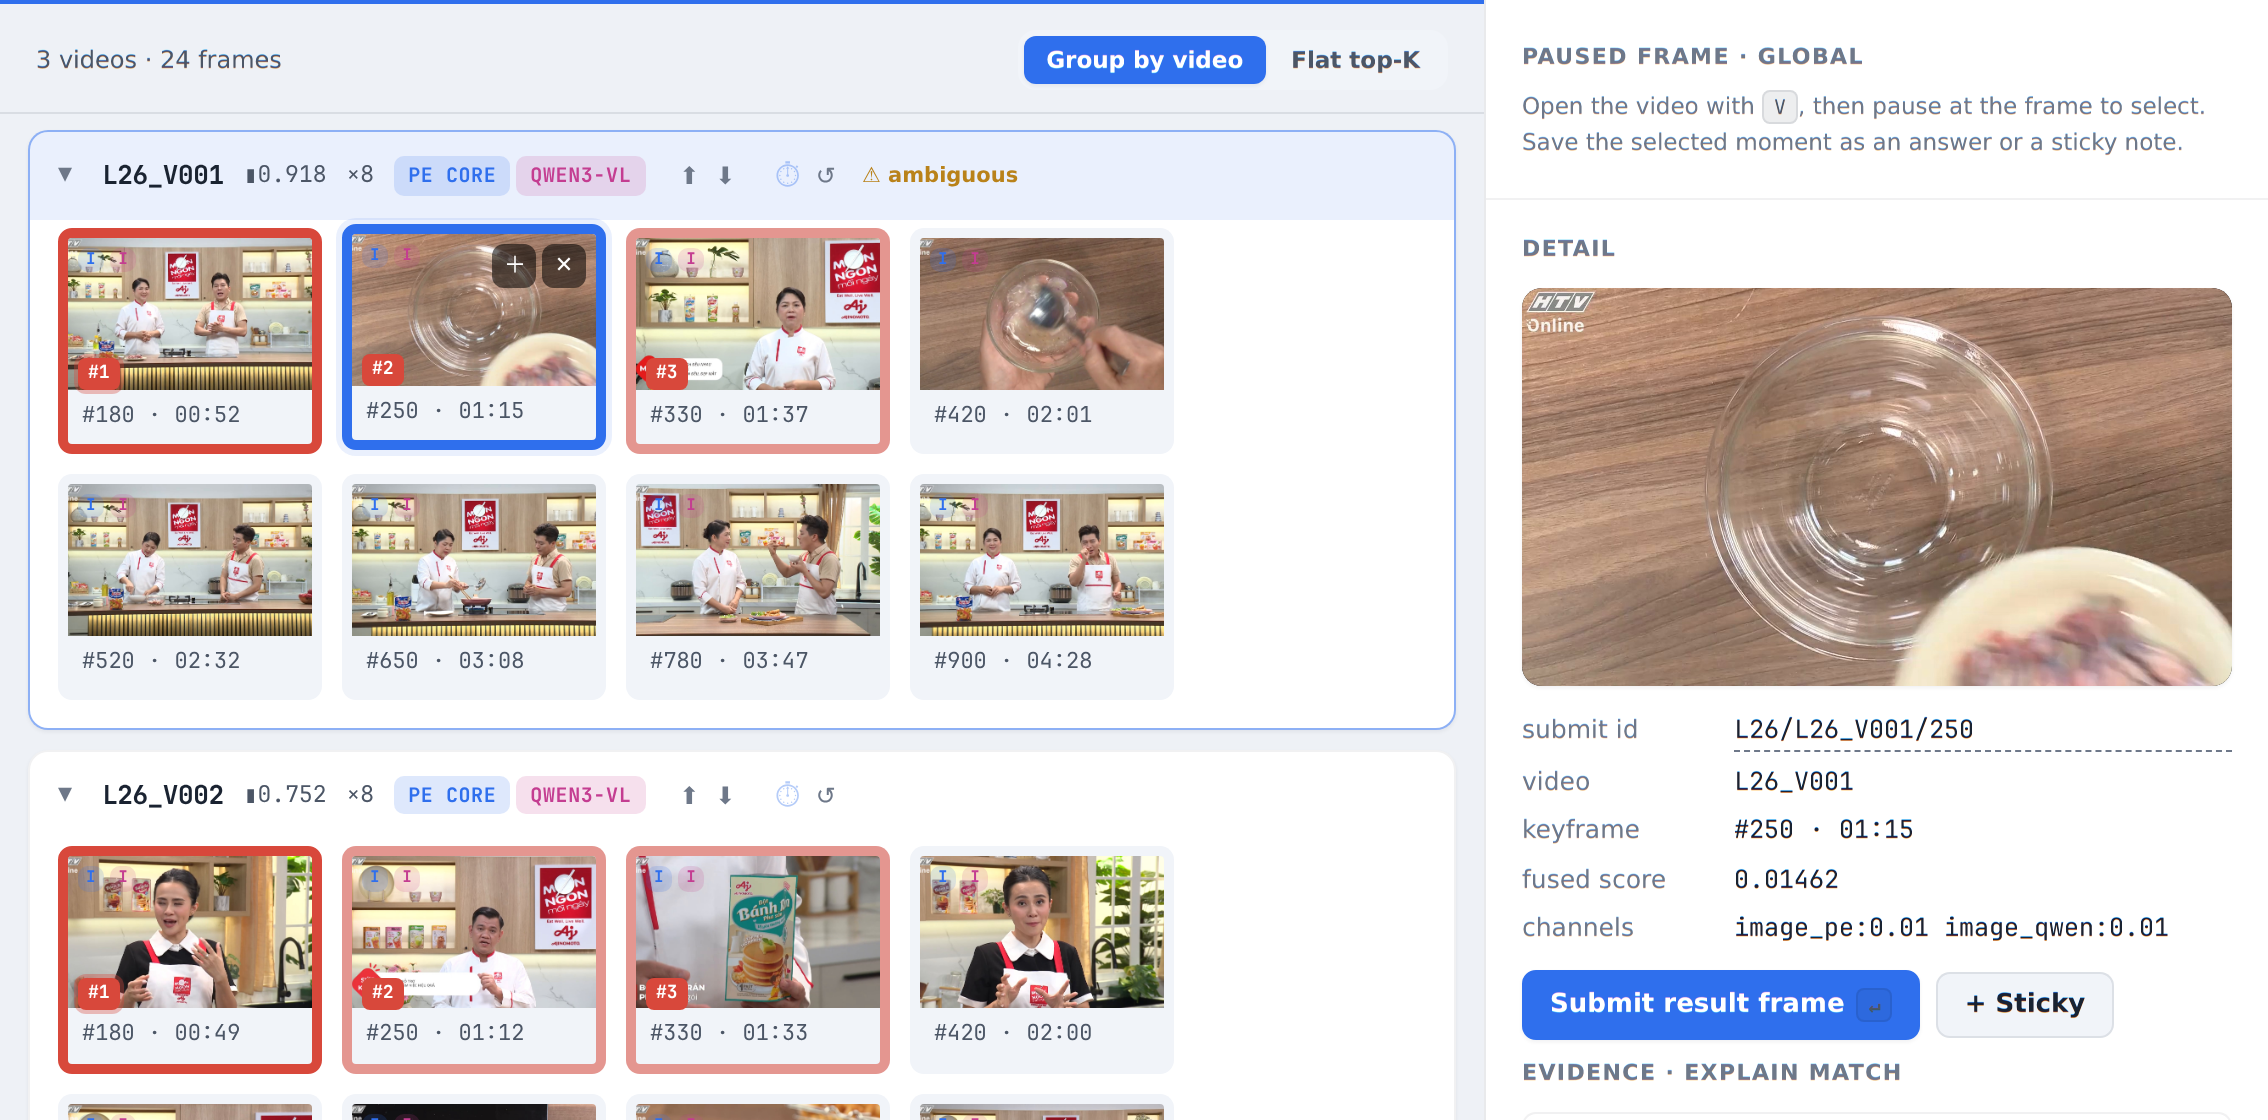
\includegraphics[width=.7\textwidth]{console-groups.png}
\caption{Console groups expose scores, frame counts, channels and ambiguity; the detail panel provides submission identifiers and evidence. Illustrative candidates use real keyframes.}
\label{fig:console}
\end{figure}

%=====================================================================
\section{CAD-VR: Evidence-Guided Fast--Slow Control}
\label{sec:cadvr}
\paragraph{Evidence board.}
Each query owns a fresh board $\mathcal{B}_t$ of constraints, candidates and evidence; no previous hint or reasoning enters it. A deterministic compiler retains the query (weight 2), extracts clauses and attribute, relation or negation spans (weight 1), and adds TRAKE events (weight 1.5) or a QA answer constraint (weight 2). Evidence is de-duplicated by kind and source. An agent's report counts as a visual observation only after that agent loaded the frame; this records inspection, not guaranteed truth. Agent confidences order that agent's proposals but are not used as probabilities.

\paragraph{Typed verification.}
Each step verifies a shortlist of five candidates, prioritising each agent's leading proposal and the verified leader, then distinct moments from the fused ranking. TRAKE can expand it to 12 to cover the leading video's events. For candidate $v$ and constraint $c$, Jev~1.13 returns a typed distribution over \{\emph{supported}, \emph{refuted}, \emph{unknown}\}, with instructions not to infer visual details from embedding scores or confidence. Here ``non-generative'' describes the decision interface: it returns probabilities rather than free-form plans or search queries. Without evidence, code sets $p^{\mathrm{sup}}=0$. It aggregates
\begin{equation}
s(v)=\exp\Bigl(\sum_{c\in\mathcal{C}(v)}w_c\log\max\bigl(\epsilon,p^{\mathrm{sup}}_c(v)\bigr)\Big/\sum_{c\in\mathcal{C}(v)}w_c\Bigr),
\label{eq:geo}
\end{equation}
a weighted geometric mean that penalises weakly supported constraints; the separate guard requires every applicable constraint to pass. \emph{Holistic} mode (E) verifies the query and answer constraints; \emph{constraint-level} mode (F) verifies all applicable constraints and enables evidence actions. Ranking promotes candidates for which \emph{supported} is the largest probability on every assessed constraint, demotes those with any \emph{refuted} maximum, and otherwise preserves fused System-1/agent order. Thus \emph{unknown} is abstention; promotion need not satisfy the stricter stop threshold.

\paragraph{Routing and the stop guard.}
While the guard fails, Jev chooses the next action from $\mathcal{A}_t\subseteq\{$\act{STOP}, \act{CALL\_CODEX}, \act{CALL\_CLAUDE}, \act{CALL\_BOTH}, \act{SEARCH\_MORE}, \act{INSPECT\_TOP1}, \act{COMPARE\_TOP2}$\}$, each described in one sentence; the first request also classifies modality and query structure. Each agent runs at most once. The evidence actions (mode F only) are backend macros: a focused search for the least-supported constraint, or OCR and speech around the top one or two candidates. Agent disagreement enters the state as a signal, and the router is told that it alone does not justify another agent. Evidence-sufficient stopping requires, for the top candidate $v_1$,
\begin{equation}
\begin{gathered}
s(v_1)\geq\tau,\qquad s(v_1)-\max_{v'\in\mathrm{comp}(v_1)}s(v')\geq\delta,\\
p^{\mathrm{sup}}_c(v_1)>\max\bigl(\tfrac12,\;p^{\mathrm{ref}}_c(v_1),\;p^{\mathrm{unk}}_c(v_1)\bigr)\ \forall c,
\end{gathered}
\label{eq:stop}
\end{equation}
where competitors exclude the same moment ($\leq8$\,s apart in one video); TRAKE compares other videos. Only scored competitors enter the maximum, which defaults to zero. QA needs an answer; TRAKE needs supported events in increasing time. We use fixed raw-score thresholds $\tau=0.9$, $\delta=0.1$. A rejected \act{STOP} triggers the next available escalation (Codex, Claude, inspect, search, compare). Budget or action exhaustion still returns the current ranking, marked separately from evidence-sufficient stopping (Algorithm~\ref{alg:cadvr}). Passing the guard is a policy decision, not a correctness guarantee.

\begin{algorithm}[t]
\caption{CAD-VR controller for one query (6 steps, 40 tool calls, 240\,s).}
\label{alg:cadvr}
\small
\begin{algorithmic}[1]
\Require query $q$, task type, System-1 result $R_0$
\State $\mathcal{C}_q\gets$ \Call{Compile}{$q$}; $\mathcal{B}_0\gets$ \Call{Seed}{$R_0,\mathcal{C}_q$}; $\mathcal{I}\gets\emptyset$ \Comment{fresh, query-local}
\For{$t=0,1,\dots$ \textbf{while} budget remains}
  \State \Call{JevVerify}{$\mathcal{B}_t$}; \Call{Publish}{ranking of $\mathcal{B}_t$}
  \If{guard~\eqref{eq:stop} holds} \Return \Comment{evidence sufficient}
  \EndIf
  \State $\mathcal{A}_t\gets\{$\act{STOP}$\}\cup\{$calls to agents $\notin\mathcal{I}\}\cup\{$untried evidence actions in mode F$\}$
  \State $a_t\gets$ \Call{JevRoute}{$\mathcal{B}_t,\mathcal{A}_t$}; \textbf{if} $a_t=$\,\act{STOP} \textbf{then} $a_t\gets$ next escalation in $\mathcal{A}_t$
  \If{$a_t=$\,\act{STOP}} \Return \Comment{actions exhausted}
  \EndIf
  \State $\mathcal{B}_{t+1}\gets$ \Call{Execute}{$a_t,\mathcal{B}_t$}; $\mathcal{I}\gets\mathcal{I}\cup$ agents in $a_t$
\EndFor
\end{algorithmic}
\end{algorithm}

\paragraph{System-2 agents and tools.}
Codex CLI with GPT-6.1 Sol~\cite{gpt61sol2026} and Claude Code with Opus 5.5~\cite{claudeopus2026} use high reasoning effort and fast mode, each in a fresh process with no shell or file tools. Both share the MCP tools in Table~\ref{tab:tools}. One-sentence soft roles favour exploration or counterexample inspection without restricting capabilities. Prompts describe the corpus and include a bounded board snapshot marked as untrusted data.

\begin{table}[t]
\caption{MCP tools shared by both agents, with mean calls per query in the initial E runs. The two local tools never search the whole corpus.}
\label{tab:tools}
\centering
\setlength{\tabcolsep}{5pt}
\scriptsize
\begin{tabular}{@{}llr@{}}
\toprule
Tool & Function & E\\
\midrule
\texttt{search} & System-1 retrieval in hybrid, visual, OCR or speech mode & 4.88\\
\texttt{list\_videos} & programme guide of a folder (speech, camera clock, race stage) & 0.98\\
\texttt{folder\_frames} & one tile per video of a folder, in a single image & 0.02\\
\texttt{video\_outline} & per-minute contents of a video (speech, text, visuals) & 0.40\\
\texttt{video\_frames} & labelled contact sheet of a time window (centre, span, density) & 4.36\\
\texttt{view\_frames} & large view of selected keyframes & 3.60\\
\texttt{video\_text} & speech and OCR text in a time window & 0.93\\
\texttt{compare\_candidates} & 2--4 moments side by side, before/centre/after, with local text & 1.17\\
\texttt{constraint\_probe} & local frames and text for one unresolved constraint & 1.05\\
\texttt{report\_candidate} & keyframe, confidence, reason, and answer or event index & 3.84\\
\bottomrule
\end{tabular}
\end{table}

%=====================================================================
\section{Experimental Setup}
\label{sec:setup}
\paragraph{Benchmark.} We assembled 111 queries from the organisers' AIC~2026 query workbooks and final-round submissions. Ground truth combines DRES-accepted submissions~\cite{dres2024} with owner-reviewed annotations, each checked against the source frames or clips: moments for all tasks, accepted answers for QA and ordered per-event alternatives for TRAKE. Queries are split by content hash and grouped by target video, so no target video appears in both DEV (25) and TEST (86). TEST has 59 T-KIS, 19 QA and 8 TRAKE queries over 87 target videos, using InfoShot++ (46 queries) or organiser (40) profiles. DEV fixed the policy; its fitted temperature calibration was not adopted. All configurations use raw probabilities.

\paragraph{Configurations.} The initial six share System-1, the soft roles and the ten tools. \textbf{A}: retrieval only. \textbf{B}: always Codex. \textbf{C}: Codex and Claude in parallel after retrieval. \textbf{D}: Jev holistic reranking without agents. \textbf{E}: CAD-VR with holistic verification. \textbf{F}: CAD-VR with constraint-level verification and evidence actions. B and C fuse retrieval and agent proposals by RRF. System-1 uses PE-Core for visual search on both profiles, heuristic parsing with VI$\to$EN translation, no LLM rewriting or reranking, and the top 150 frames in at most 30 videos; routing activated OCR in 18, speech in 11, audio in 9 and TARA in 5 TEST queries.

\paragraph{Metrics.} \emph{Strict} R@$k$ and MRR require a moment within $\pm1$\,s; QA additionally requires a normalised accepted answer, and TRAKE a complete ordered sequence in one video. \emph{Video} R@$k$ checks target identity among the first $k$ distinct videos. \emph{Group-moment} R@$k$ checks whether those videos contain a returned matching moment, ignoring QA answers but retaining TRAKE's complete-sequence requirement. Video order follows first occurrence in the saved ranking. Rescue@1 measures strict success with agent provenance among runs whose own retrieval seed failed. We record latency, calls and tokens, plus ECE (10 bins) and Brier score~\cite{brier1950} over final scored candidates of non-TRAKE queries. Reliability plots use five bins; candidate observations are not independent query samples.

\paragraph{Protocol.} Each query--configuration pair is a fresh live run, with variants in seeded random order per query. The initial comparison retains 516 completed TEST runs. The supplementary C/C+V/E round uses the same 86 queries (258 runs), raw policy, prompts, tools, retrieval and budgets. C+V adds E's final holistic verifier to C, with no routing or adaptive stopping, and saves pre-verification rankings. This separate round reuses analysed TEST data without new DEV tuning.

Quota-interrupted attempts are archived and retried from fresh state. The supplementary round has no completed-run errors/fallback. Its 13 interruptions add 314.6\,s and 25 agent calls, excluding pauses; tables report completed-attempt latency. Percentile bootstrap intervals~\cite{efron1979} resample base queries: 2,000 draws for initial per-configuration intervals and 10,000 paired draws (seed 2026) for contrasts. Exact McNemar tests~\cite{mcnemar1947} complement these exploratory, multiplicity-uncorrected comparisons. Code and reproducibility artifacts, including benchmark manifests, configuration hashes, and query-level evaluation reports, are available at the \href{https://github.com/vonhatbao2205/AIC2026/tree/main/benchmarks/agent}{GitHub benchmark directory}\footnote{\url{https://github.com/vonhatbao2205/AIC2026/tree/main/benchmarks/agent}}. Competition media are not redistributed.

%=====================================================================
\section{Results}
\label{sec:results}
\subsection{Initial Six-Configuration Comparison}
E has the highest observed strict R@1 in Table~\ref{tab:main} (58.1\%). E improves on B by 18.6 points (95\% CI $[9.3,27.9]$; McNemar $p<0.001$). Its E--C difference is inconclusive ($+7.0$, $[-2.3,16.3]$; 11 E-only and 5 C-only successes, $p=0.21$). C has the highest R@5 (72.1\% vs.\ 67.4\%).

D equals A on retrieval accuracy metrics: all 525 assessments were \emph{unknown}, preserving System-1 order. This shows no gain from verification of retrieval-only evidence in this setting; it does not isolate verification after agent inspection. F does not improve overall on E ($-5.8$ points, $[-15.1,3.5]$), and changes both verification granularity and available evidence actions.

\begin{table}[t]
\caption{Initial TEST round (N=86; tolerance 1\,s). R@1: bootstrap 95\% CI, 2,000 draws; Resc.: Rescue@1, 73 eligible runs/variant; p50: median latency; Agents: invocations/query; kTok: mean agent and decision tokens in thousands.}
\label{tab:main}
\centering
\setlength{\tabcolsep}{3.1pt}
\footnotesize
\begin{tabular}{@{}llcccccrr@{}}
\toprule
& Configuration & R@1 [95\% CI] & R@5 & MRR & Resc. & p50 (s) & Agents & kTok\\
\midrule
A & Retrieval only & 15.1 [8.1, 23.3] & 33.7 & .233 & -- & 1.6 & 0 & 0\\
D & Jev rerank & 15.1 [8.1, 23.3] & 33.7 & .233 & 0.0 & 2.1 & 0 & 3\\
B & Always Codex & 39.5 [29.1, 50.0] & 68.6 & .529 & 28.8 & 50.5 & 1.00 & 230\\
C & Always both & 51.2 [40.7, 61.6] & \textbf{72.1} & .612 & 42.5 & 51.2 & 2.00 & 323\\
\midrule
E & CAD-VR, holistic & \textbf{58.1} [47.7, 68.6] & 67.4 & \textbf{.630} & \textbf{52.1} & 72.6 & 1.95 & 316\\
F & CAD-VR, constraint & 52.3 [41.9, 62.8] & 64.0 & .572 & 45.2 & 84.2 & 1.99 & 416\\
\bottomrule
\end{tabular}
\end{table}


F leads initial TRAKE R@1 (50.0\% versus E's 37.5\% and C's 25.0\%), but eight queries make this suggestive only.

\subsection{Live C/C+V/E Ablation}
\label{sec:ablation}
Table~\ref{tab:cv} tests final verification after always-two acquisition. All 86 C+V traces show both agents, one final verification and no routing. C+V--C and E--C+V remain inconclusive. E--C is positive in this round (unadjusted $p=0.035$), unlike the initial round, but does not establish a gain over the C+V control.

\begin{table}[t]
\caption{Supplementary TEST round (N=86); recall in percent. Lower panel: paired R@1 contrasts, 95\% bootstrap CIs (10,000 draws), exact unadjusted McNemar $p$ and discordant win/loss counts. ``Pre'': C+V's own ranking before verification.}
\label{tab:cv}
\centering
\footnotesize
\setlength{\tabcolsep}{5pt}
\begin{tabular}{@{}lrrrrrrr@{}}
\toprule
& R@1 & R@5 & MRR & p50 (s) & p95 (s) & Agents & Jev calls\\
\midrule
C & 47.7 & \textbf{69.8} & .579 & 53.7 & 103.2 & 2.00 & 0.00\\
C+V & 50.0 & 66.3 & .581 & 55.6 & 98.4 & 2.00 & 1.00\\
E & \textbf{58.1} & 66.3 & \textbf{.620} & 75.8 & 198.9 & 1.95 & 4.91\\
\bottomrule
\end{tabular}
\smallskip

\begin{tabular}{@{}lrrr@{}}
\toprule
Contrast & $\Delta$R@1 (pp) [95\% CI] & Win/loss & $p$\\
\midrule
C+V $-$ C & $+2.3\;[-3.5,9.3]$ & 5/3 & .727\\
E $-$ C+V & $+8.1\;[0.0,16.3]$ & 10/3 & .092\\
E $-$ C & $+10.5\;[2.3,18.6]$ & 12/3 & .035\\
C+V $-$ Pre & $+3.5\;[-1.2,9.3]$ & 4/1 & .375\\
\bottomrule
\end{tabular}
\end{table}

C/C+V use identical acquisition policies but independent trajectories. E--C+V is a controller-package contrast: scheduling, intermediate verification, board-conditioned context and stopping vary together. By task, C/C+V/E obtain 57.6/61.0/74.6\% T-KIS, 26.3/26.3/31.6\% QA and 25.0/25.0/0.0\% TRAKE R@1. E's unchanged aggregate 58.1\% across rounds therefore hides task-level variability, including the loss of its three initial TRAKE successes.

\subsection{What Does Final Verification Contribute?}
\label{sec:ranking-diagnostic}
On identical C+V candidates and answers, final verification raises R@1 from 40/86 (46.5\%) to 43/86 (50.0\%): four repairs and one harm. This same-evidence difference is inconclusive (Table~\ref{tab:cv}).

For the initial E/F runs, a complementary offline diagnostic sorts final candidates by logged RRF score, first-seen time and keyframe identifier. This reproduces all 344 A/B/C/D rankings. E's RRF order yields 51/86 (59.3\%) versus the logged 50/86 (58.1\%): one repair, two harms; F yields 48/86 (55.8\%) versus 45/86 (52.3\%): one repair, four harms. Neither difference is conclusive (95\% CIs $[-5.8,2.3]$ and $[-9.3,1.2]$ points). These mixed results limit general reranking claims; earlier verification may still affect acquisition and context.

\subsection{Accuracy, Latency and Computation}
In the initial round, CAD-VR did not save computation (Fig.~\ref{fig:tradeoff}): E invoked 1.95 agents per query, and its median latency (72.6\,s; p95 171\,s) exceeds C's (51.2\,s; p95 94\,s). The router sent the investigator first in 83/86 queries; sequential escalation adds agent times. Jev averaged 4.9 calls and 3.2\,s/query (Fig.~\ref{fig:controller}a). The supplementary round confirms this pattern (Table~\ref{tab:cv}); E/C+V/C use 327k/344k/346k tokens. Calls and tokens are workload proxies, not FLOPs or complete financial cost.

\begin{figure}[t]
\centering
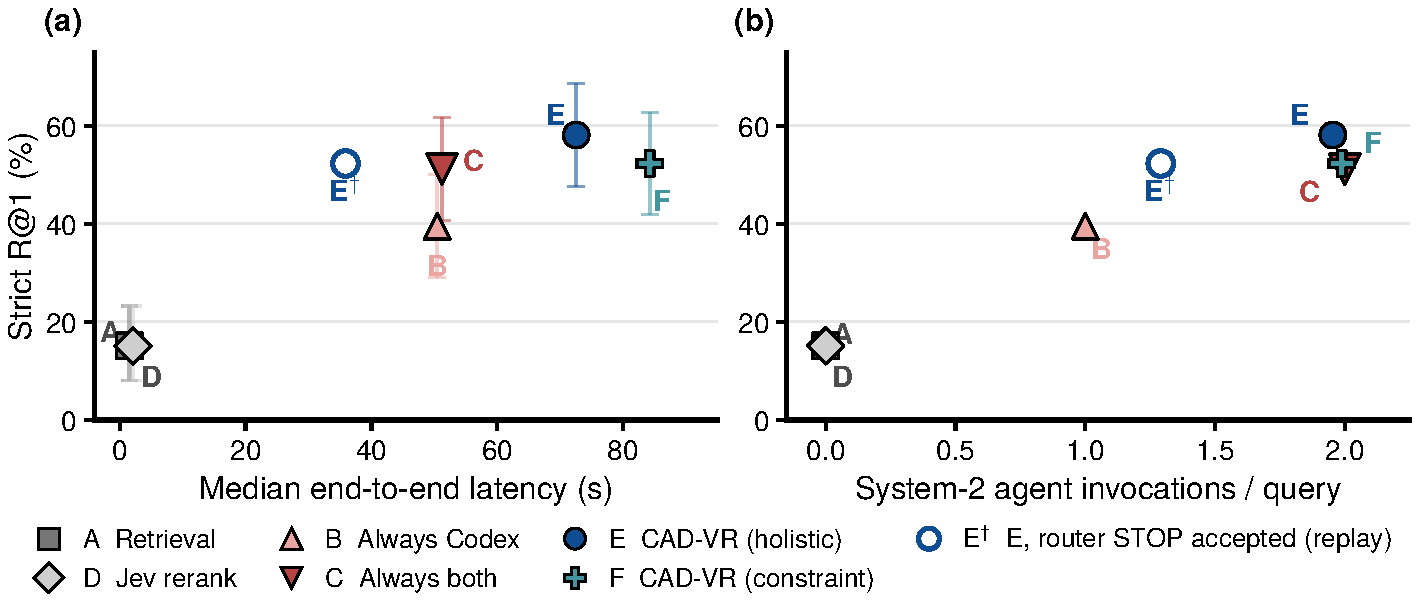
\includegraphics[width=\textwidth]{tradeoff.pdf}
\caption{Initial-round strict R@1 versus latency (a; 95\% bootstrap CIs) and agent calls (b). E$^\dagger$ is an offline first-\act{STOP} replay, not a deployed configuration (Sect.~\ref{sec:controller}).}
\label{fig:tradeoff}
\end{figure}

\subsection{What Controls Compute: Router versus Guard}
\label{sec:controller}
In the initial E traces, after the first agent returned, the router proposed \act{STOP} with probability above 0.5 in 57 of 82 decisions (median 0.73). The top-1 was already correct in 31 of those 57 queries, versus 7 of the other 25 (Fig.~\ref{fig:controller}b). The guard overrode all 57 proposals; only 9 runs ended with sufficient evidence. In a post-hoc replay (E$^\dagger$), we retain the ranking published immediately before the first router \act{STOP} and truncate calls and elapsed time there; runs without a proposal retain their final outcome. This yields 1.29 agents/query, 35.9\,s median logged latency and 52.3\% R@1, versus deployed E's 1.95, 72.6\,s and 58.1\%. Replay fixes earlier TEST decisions; its timing is not live measurement. Numerical proximity to C does not establish equivalence or validate efficiency. A deployable policy requires DEV selection and new live evaluation.

Verifier scores are imperfect proxies for strict correctness (ECE 0.106, Brier 0.112; Fig.~\ref{fig:controller}c): only 7 of 13 candidates scored at least 0.8 were correct. This diagnostic compares evidence support with strict moment/answer labels, not human-labelled constraint support. Neither the raw score nor the additional guard terms guarantee correctness. A revised stop policy would require development-only selection and a new held-out live evaluation.

\begin{figure}[t]
\centering
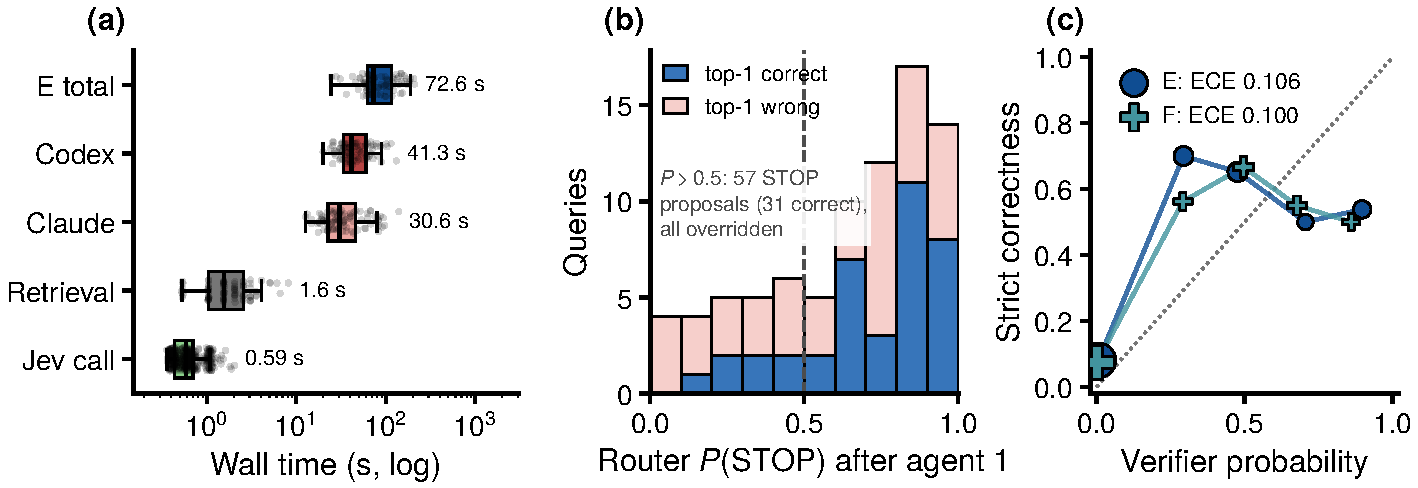
\includegraphics[width=\textwidth]{controller.pdf}
\caption{Initial controller diagnostics. (a) E wall time per layer (log scale). (b) Router $P(\mathrm{STOP})$ after agent 1 by top-1 correctness; every proposal above 0.5 was overridden. (c) E/F verifier reliability (marker area $\propto$ count).}
\label{fig:controller}
\end{figure}

\subsection{Group-by-Video Evaluation}
Figure~\ref{fig:grouping} separates exact-answer accuracy from coverage in the returned video groups. Retrieval has strict, group-moment and video R@1 of 15.1\%, 43.0\% and 45.3\%; E reaches 58.1\%, 81.4\% and 86.0\%. Group-moment R@5 is 86--90\% for the agent configurations. These same-ranking metric gaps motivate browsing, not a claimed gain over ungrouped retrieval. QA's 89.5\% group-moment versus 42.1\% strict R@1 for E combines two effects, selecting the exact frame and supplying an accepted answer. Neither answer extraction alone nor operator effort is isolated.

\begin{figure}[t]
\centering
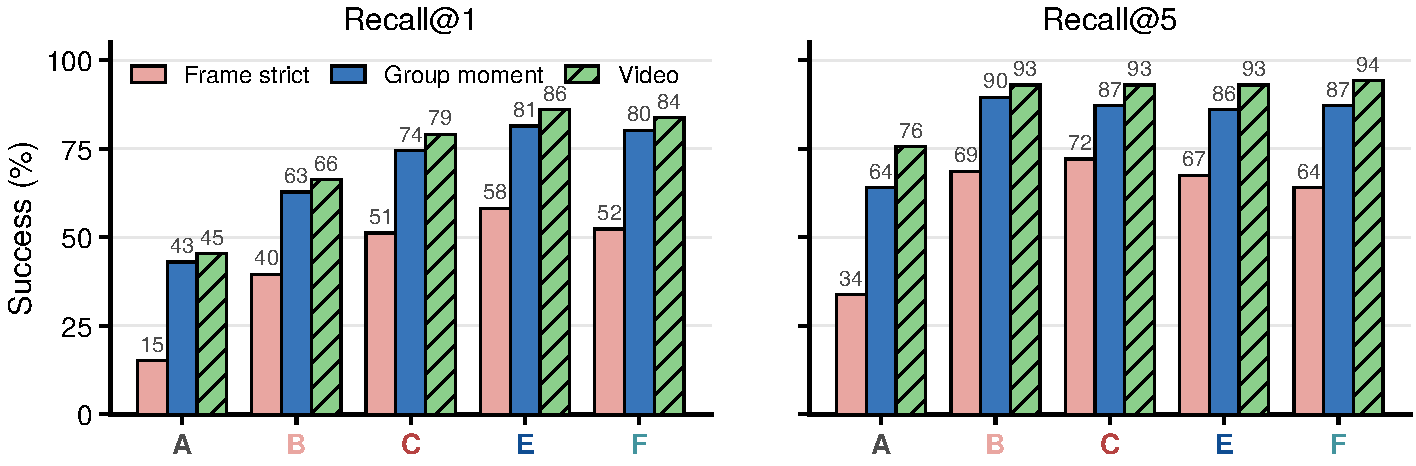
\includegraphics[width=\textwidth]{grouping.pdf}
\caption{Initial strict, group-moment and video R@$k$ (D=A). Group-moment checks evidence in the first $k$ videos, ignoring QA answers but requiring complete TRAKE sequences. This compares metrics, not grouping algorithms.}
\label{fig:grouping}
\end{figure}

\subsection{Cumulative-Hint Evaluation}
Twenty-four TEST queries (12 T-KIS, 12 QA) have three or four reviewed hints whose concatenation equals the full query. Each prefix $h_1$, $h_1{+}h_2$, \dots\ is an \emph{independent} query run from a fresh state, without cross-hint memory or any progressive mechanism; we compare A, C and F. With only the first hint (Fig.~\ref{fig:cumulative}a), F ranks the target video first for 83.3\% of queries, against 66.7\% for C ($+16.7$ points, $[4.2,33.3]$) and 41.7\% for A. On the full query, strict R@1 is 41.7\%, 33.3\% and 12.5\% (F vs.\ A $+29.2$, $[12.5,50.0]$; F vs.\ C $+8.3$, $[-8.3,25.0]$). F uses 1.79 agents at $h_1$ versus 2.0 at full, and 9.2 versus 12.3 Jev calls. Its early video success is 95.8\% (Table~\ref{tab:hints}); first-success prefixes are retrospective and later prefixes may fail again.

\begin{figure}[t]
\centering
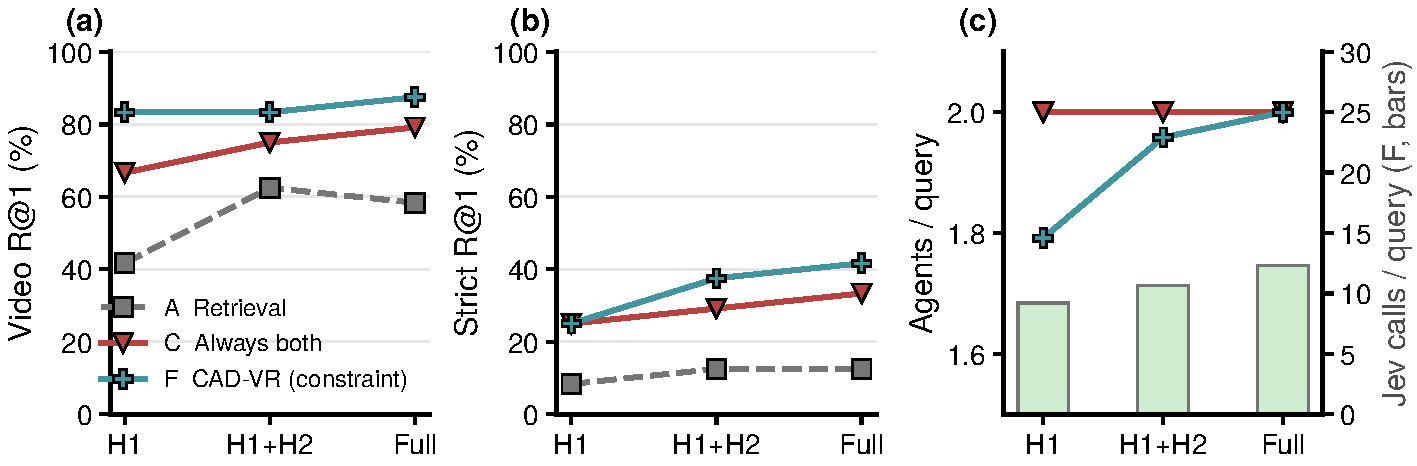
\includegraphics[width=\textwidth]{cumulative.pdf}
\caption{Cumulative-hint evaluation on 24 TEST queries, each prefix a fresh, independent run. (a) Video R@1. (b) Strict R@1. (c) Agents per query (lines) and Jev calls per query for F (bars).}
\label{fig:cumulative}
\end{figure}

\begin{table}[t]
\caption{Hints-to-solve on 24 queries. $h^\star$: first successful prefix ($H{+}1$ if unsolved); Early: success before the last hint; Hint saving: $(H-h^\star)/(H-1)$, 0 if unsolved. These retrospective measures do not imply online stopping or compute savings.}
\label{tab:hints}
\centering
\setlength{\tabcolsep}{3.8pt}
\footnotesize
\begin{tabular}{@{}lcccccccc@{}}
\toprule
& \multicolumn{4}{c}{Video criterion} & \multicolumn{4}{c}{Strict criterion}\\
\cmidrule(lr){2-5}\cmidrule(l){6-9}
& Solved & Mean $h^\star\downarrow$ & Early & Hint saving & Solved & Mean $h^\star\downarrow$ & Early & Hint saving\\
\midrule
A & 19 & 2.25 & .750 & .611 & 6 & 4.04 & .250 & .153\\
C & 22 & 1.67 & .875 & .792 & 10 & 3.42 & .375 & .319\\
F & \textbf{23} & \textbf{1.38} & \textbf{.958} & \textbf{.889} & \textbf{12} & \textbf{3.25} & \textbf{.458} & \textbf{.361}\\
\bottomrule
\end{tabular}
\end{table}

\subsection{Qualitative Example}
Figure~\ref{fig:example} traces an initial-round TEST query through E. Retrieval finds the right video but an interview scene. Claude finds the feeding moment; Jev supports it (0.73) and refutes a near-duplicate (0.81). The router proposes \act{STOP} (0.97), but the guard rejects it ($0.73<\tau$), triggering Codex's local inspection.

\begin{figure}[t]
\centering
\resizebox{\textwidth}{!}{% Qualitative TEST example T-KIS:query-p1-5-kis (target L27_V014, frames 634/675 @25 fps).
% Times, probabilities and tool counts are copied from the logged E/C/A runs in
% benchmarks/agent/runs/soict-final-dev-test-pooled-tol1-v1/test/main/results.jsonl.
\definecolor{csInk}{HTML}{243449}
\definecolor{csBlue}{HTML}{286A9B}
\definecolor{csTeal}{HTML}{1F7A70}
\definecolor{csAmber}{HTML}{B5651D}
\definecolor{csRed}{HTML}{B64342}
\definecolor{csGreen}{HTML}{2E7D32}
\begin{tikzpicture}[x=1cm,y=1cm,font=\fontfamily{qhvc}\fontsize{6.2}{7.3}\selectfont,text=csInk,
 capt/.style={font=\fontfamily{qhvc}\fontsize{6}{7}\selectfont,align=left,anchor=north west,inner sep=0pt,text width=3.85cm},
 tag/.style={font=\fontfamily{qhvc}\bfseries\fontsize{6.2}{7.3}\selectfont,anchor=south west,inner sep=1.4pt},
 ev/.style={font=\fontfamily{qhvc}\fontsize{5.6}{6.5}\selectfont,align=center,inner sep=.8pt}]
% ---------------- query ----------------
\node[draw=black!25,fill=black!3,rounded corners=1.6pt,text width=11.95cm,align=left,inner sep=3pt,anchor=north west] (q) at (0,0)
 {\textbf{T-KIS query} (Vietnamese, translated): \emph{Two women are feeding goats: one wears a white T-shirt with a red shirt draped
 over her shoulders, the other a traditional purple striped long-sleeved top. Both smile and look delighted. A spacious farm with a
 corrugated-iron roof and wooden fences dividing rows of pens, holding a long row of goats.}};
% ---------------- three candidates ----------------
\foreach \k/\x/\name/\col/\mark in {855/0/A\ \ System-1 top-1/csRed/\faTimes, 1060/4.08/C\ \ always-two top-1/csRed/\faTimes, 145/8.16/E\ \ CAD-VR top-1/csGreen/\faCheck} {
  \node[inner sep=0pt,anchor=north west,draw=\col,line width=1.1pt] (img\k) at (\x,-0.98) {\includegraphics[width=3.85cm]{keyframes/L27_V014_\k_640.jpg}};
  \node[tag,fill=white,text=\col] at (img\k.south west) {\mark\ \name};
}
\node[capt] at (0,-3.25) {\textbf{3:55}, correct video, wrong moment (interview).\\Strict rank of the target: 18.};
\node[capt] at (4.08,-3.25) {\textbf{4:55}, near-duplicate: same pair, but the woman\\in white is talking. Both agents reported it; RRF\\placed it first. In E, Jev: \emph{refuted} 0.81.};
\node[capt] at (8.16,-3.25) {\textbf{0:26}, all clauses hold (target 0:25.4--0:27.0).\\Claude 0.82, Codex 0.92; Jev: \emph{supported} 0.73\\after Claude, 0.60 at the end. Strict rank 1.};
% ---------------- timeline of the E run ----------------
\def\s{0.1625}% cm per second, 0..72 s
\begin{scope}[shift={(0.25,-4.75)}]
 \draw[-{Stealth[length=1.3mm]},line width=.5pt,draw=black!60] (0,0) -- (72*\s+0.2,0) node[right,ev] {s};
 \foreach \t in {0,10,...,70} { \draw[draw=black!60,line width=.4pt] (\t*\s,0) -- (\t*\s,-0.06) node[below,ev,text=black!60] {\t}; }
 % agent work spans
 \fill[csAmber!25,draw=csAmber!70,line width=.4pt,rounded corners=.8pt] (3.71*\s,0.07) rectangle (21.19*\s,0.33);
 \node[ev,text=csAmber!80!black] at (12.45*\s,0.2) {\textbf{Claude} 17.5 s, 5 tools};
 \fill[csAmber!12,draw=csAmber!70,line width=.4pt,rounded corners=.8pt] (22.25*\s,0.07) rectangle (69.81*\s,0.33);
 \node[ev,text=csAmber!80!black] at (46.0*\s,0.2) {\textbf{Codex} 47.6 s, 10 tools incl.\ \texttt{constraint\_probe}(``both women smiling'')};
 % controller events
 \foreach \t in {2.73,3.71,21.83,22.25,71.25} { \fill[csTeal] (\t*\s,0) circle (1.1pt); }
 \draw[csTeal,line width=.4pt] (2.73*\s,0) -- (0.0,0.62) node[above,ev,anchor=south west,text=csInk] {\textbf{2.7 s} retrieval seeds board};
 \draw[csTeal,line width=.4pt] (3.71*\s,0) -- (1.05,0.42) node[above,ev,anchor=south west,text=csInk,xshift=3pt] {\textbf{3.7 s} Jev route: \texttt{CALL\_CLAUDE} (0.80); visual, compositional};
 \draw[csTeal,line width=.4pt] (21.83*\s,0) -- (3.40,-0.34) node[ev,anchor=north east,text=csInk] {\textbf{21.8 s} Jev verify: 0:26 \emph{sup} 0.73, 4:55 \emph{ref} 0.81};
 \draw[csTeal,line width=.4pt] (22.25*\s,0) -- (3.95,-0.34) node[ev,anchor=north west,text=csInk] {\textbf{22.3 s} router \emph{P}(STOP)\,=\,0.97, but guard fails (0.73\,<\,$\tau$)\,$\Rightarrow$\,\texttt{CALL\_CODEX}};
 \draw[csTeal,line width=.4pt] (71.25*\s,0) -- (11.55,0.42) node[above,ev,anchor=south east,text=csInk] {\textbf{71.2 s} final verify, 0:26 top-1};
\end{scope}
\end{tikzpicture}
}
\caption{Initial-round TEST example. Top: top-1 frames of retrieval (A), always-two (C) and CAD-VR (E). Bottom: E's logged controller events (teal) and agent work (amber). The left frame's lower-third is blurred.}
\label{fig:example}
\end{figure}

\FloatBarrier

%=====================================================================
\section{Discussion and Limitations}
\label{sec:discussion}
\paragraph{Component attribution.} C+V supplies the missing final-verifier control, but E--C+V remains inconclusive. Nonsignificance does not establish equivalence. Mixed ranking effects do not establish a general reranking benefit, and scheduling alone remains unisolated.

\paragraph{Compute.} The guard prioritises auditable evidence sufficiency over compute reduction. Both rounds show negligible call reduction and higher E latency. Development-selected stopping and parallel escalation require live evaluation; replay is diagnostic.

\paragraph{Validity.} The small Vietnamese corpus and owner-reviewed labels limit generalisation and annotation independence. Video-disjoint splits retain thematic overlap; bootstraps omit shared-video dependence. Two rounds expose but do not reliably estimate C/E variability; C+V has one run per query, on an already analysed TEST set. Hosted services cannot be frozen by identifiers. F jointly changes granularity and actions. Text-only verification inherits observation errors; geometric support is not calibrated joint correctness. Group weights are unablated; operator effort is unmeasured.

%=====================================================================
\section{Conclusion}
\label{sec:conclusion}
CAD-VR exposes auditable escalation and stopping through typed control and a query-local evidence board. E leads observed R@1 in both rounds, but its increment over C+V remains inconclusive. Ranking effects are mixed; neither round shows practical compute savings. Group and independent-hint analyses distinguish coverage from exact answers. Stronger causal or efficiency claims require repeated evaluation and development-selected stopping.

\bibliographystyle{splncs04}
\bibliography{references}
\end{document}
